
\documentclass[12pt]{article}

\usepackage[a4paper,margin=1in]{geometry}
\usepackage{graphicx}
\usepackage{titlesec}
\usepackage{setspace}
\usepackage{float} % prevents figures from floating

\titleformat{\section}{\large\bfseries}{\thesection.}{0.5em}{}

\begin{document}

\begin{center}

{\Large \textbf{Industrial Motor Condition and Energy Monitoring System using IoT}}

\vspace{0.3cm}

Bhuvnesh Verma, Aryan Bokde

\vspace{0.2cm}

Department of Artificial Intelligence and Cyber Security,\\
Ramdeobaba University, Nagpur, India.

\vspace{0.2cm}

Email: bhuvneshverma2904@gmail.com, aryanbokde210105@gmail.com

\end{center}

\vspace{0.5cm}

\textbf{Abstract}

This paper presents an IoT-based Industrial Motor Condition and Energy Monitoring System designed to improve reliability, reduce energy wastage, and enable predictive maintenance in industrial environments. The system continuously monitors parameters such as motor current, temperature, vibration, and energy consumption using sensors connected to an ESP32 microcontroller. Data is transmitted to a cloud-based dashboard for real-time visualization and analysis. Alerts are generated whenever abnormal operating conditions are detected, enabling early fault detection and reducing unexpected downtime. The proposed system provides a cost-effective and scalable solution for industrial automation and smart energy management.

\vspace{0.3cm}

\textbf{Keywords:} IoT, Industrial Motor Monitoring, Energy Monitoring, Predictive Maintenance, ESP32.

\vspace{0.4cm}

\section{Introduction}

Industrial motors are widely used in manufacturing plants, pumping stations, and production lines. Unexpected motor failures can cause production losses, safety risks, and increased maintenance costs. Traditional monitoring methods rely on manual inspection, which is inefficient and may fail to detect early signs of faults. The Internet of Things (IoT) enables real-time monitoring of equipment through interconnected sensors and cloud platforms.

By integrating sensors with microcontrollers and wireless communication technologies, industrial parameters such as temperature, vibration, and current can be continuously monitored. In this work, an IoT-based monitoring system is proposed to track motor health and energy consumption.

\section{Literature Review}

Recent research highlights the growing use of IoT in industrial monitoring systems. Several studies have proposed wireless sensor networks to track machine health parameters such as vibration and temperature. Smart monitoring platforms using ESP32, Arduino, and cloud services allow engineers to monitor machine conditions remotely.

Energy monitoring systems using current sensors have also been implemented to analyze power consumption and improve energy efficiency in industrial equipment.

\section{Methodology}

The proposed system uses sensors to monitor motor parameters such as current, temperature, and vibration. These sensors are connected to an ESP32 microcontroller that processes the collected data. The processed data is transmitted to an IoT cloud platform where it is visualized through dashboards and graphs.

If any parameter exceeds predefined thresholds, alerts are generated to notify operators.

\begin{figure}[H]
\centering
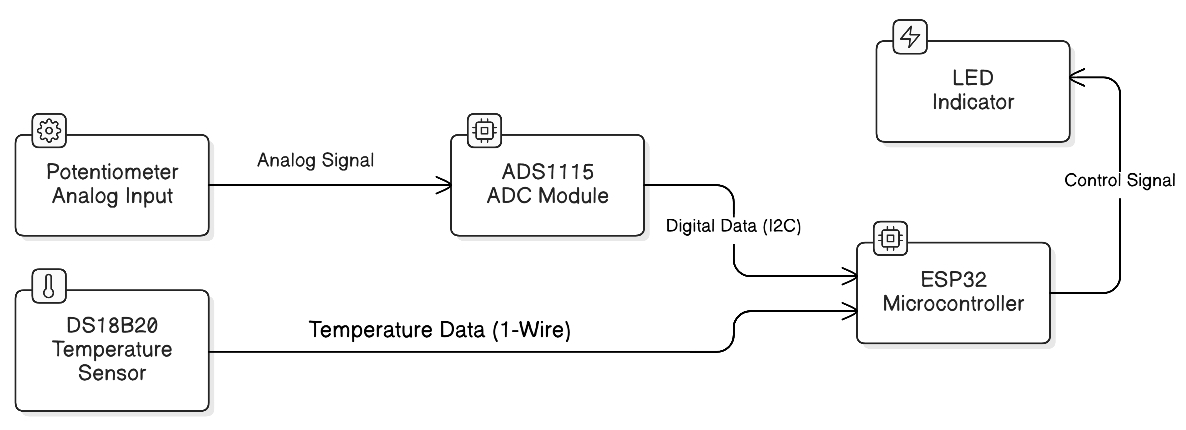
\includegraphics[width=0.6\textwidth]{images/sys.jpeg}
\caption{System architecture of the Industrial Motor Condition and Energy Monitoring System}
\end{figure}

\begin{figure}[H]
\centering
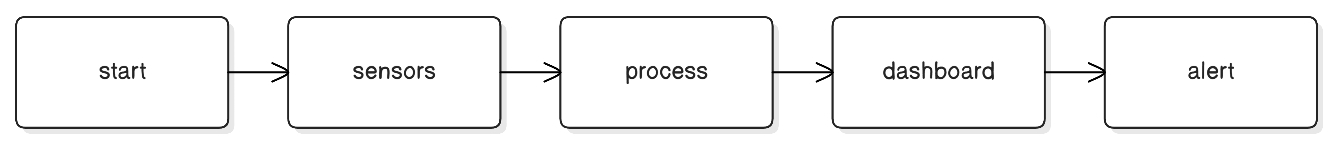
\includegraphics[width=0.6\textwidth]{images/flow.jpeg}
\caption{Flowchart of the proposed monitoring system}
\end{figure}

\section{Prototype Design and Hardware Integration}

The prototype consists of an ESP32 microcontroller, current sensor (ACS712), temperature sensor (DS18B20), vibration sensor, and Wi-Fi connectivity. The sensors measure real-time parameters of the motor and send them to the ESP32 for processing.

The ESP32 transmits the data to an IoT platform such as ThingsBoard or Blynk. The dashboard displays real-time values, historical graphs, and alerts whenever abnormal conditions are detected.

\section{Results and Discussion}

The system was tested under various operating conditions to analyze motor performance and energy consumption. The IoT dashboard successfully displayed real-time data and generated alerts whenever abnormal conditions were detected.

\begin{figure}[H]
\centering
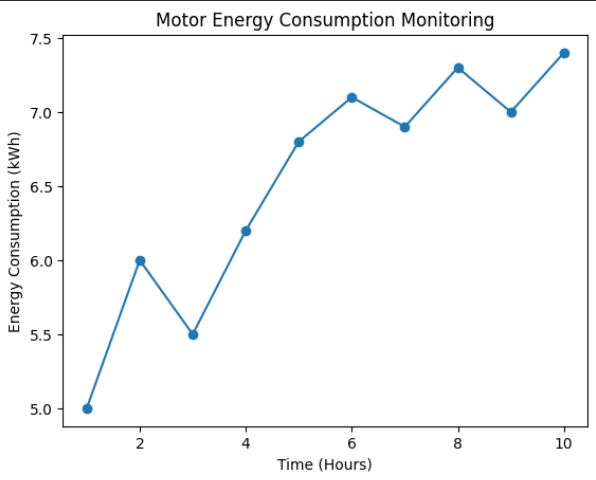
\includegraphics[width=0.6\textwidth]{images/energy_monitoring.jpeg}
\caption{Energy consumption monitoring of the motor}
\end{figure}

\begin{figure}[H]
\centering
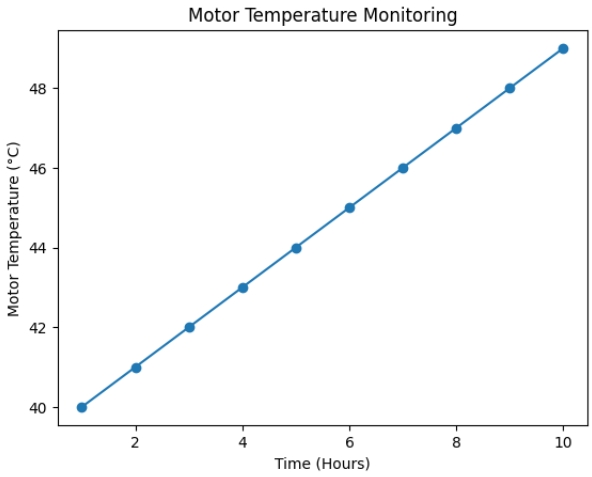
\includegraphics[width=0.6\textwidth]{images/temperature_monitoring.jpeg}
\caption{Motor temperature monitoring results}
\end{figure}

The results demonstrate that the system is capable of monitoring key motor parameters accurately and providing early warnings in case of abnormal conditions.

\section{Conclusion}

This paper presented an IoT-based Industrial Motor Condition and Energy Monitoring System capable of monitoring important parameters such as temperature, vibration, and energy consumption. The system enables real-time monitoring, early fault detection, and improved energy management.

The prototype demonstrated reliable performance and can be extended for predictive maintenance in large-scale industrial environments.

\section{References}

[1] Smith, J., “IoT-Based Industrial Equipment Monitoring Systems,” IEEE, 2022.

[2] Kumar, A., “Energy Monitoring in Smart Industries using IoT,” Elsevier, 2023.

[3] Patel, R., “Predictive Maintenance using Sensor Networks,” Springer, 2021.

\end{document}
```
